\section{Iteration Keyword}

%\begin{figure}[t]
%{\eightpoint
%\begin{verbatim}
%  int->int stateful filter SingleInductionFilter() {
%      int counter;
%      int max;
%  
%      work push 1 pop 1{
%
%          ...
%
%          counter = (counter + C);
%
%          if (counter > max) {
%              counter = 0;
%          } 
%      }
%  }
%\end{verbatim}
%\caption{Stateful StreamIt filter using induction variable state.\protect\label{fig:transform-before-simple}}}
%\end{figure}
%
%\begin{figure}[t]
%{\eightpoint
%\begin{verbatim}
%  int->int filter SingleInductionFilter() {
%      int max;
%  
%      work push 1 pop 1{
%          int counter = (iter() * C) % max;
%
%          ...
%
%      }
%  }
%\end{verbatim}
%\caption{Stateless StreamIt filter using iteration keyword.\protect\label{fig:transform-after-simple}}}
%\end{figure}
%
%
%\begin{figure}[t]
%{\eightpoint
%\begin{verbatim}
%  int->int stateful filter StartingValueInductionFilter() {
%      int counter;
%      int start;
%      int max;
%
%      init {
%          counter = start;
%      }
%  
%      work push 1 pop 1{
%
%          ...
%
%          counter = (counter + 1);
%
%          if (counter > max) {
%              counter = start;
%          } 
%      }
%  }
%\end{verbatim}
%\caption{Stateful StreamIt filter using induction variable state starting at and resetting to a special starting value.\protect\label{fig:transform-before-starting}}}
%\end{figure}
%
%\begin{figure}[t]
%{\eightpoint
%\begin{verbatim}
%  int->int filter StartingValueInductionFilter() {
%      int max;
%      int start;
%  
%      work push 1 pop 1{
%          int counter = iter() % (max - start) + start;
%
%          ...
%
%      }
%  }
%\end{verbatim}
%\caption{Stateless StreamIt filter using iteration keyword starting at and resetting to a special starting value.\protect\label{fig:transform-after-starting}}}
%\end{figure}
%
%\begin{figure}[t]
%{\eightpoint
%\begin{verbatim}
%  int->int stateful filter TwoNestedInductionFilter() {
%      int counter_x;
%      int counter_y;
%      int max_x;
%      int max_y;
%  
%      work push 1 pop 1{
%
%          ...
%
%          counter_x = (counter_x + 1);
%
%          if (counter_x > max_x) {
%              counter_x = 0;
%              counter_y = (counter_y + 1);
%
%              if (counter_y > max_y) {
%                  counter_y = 0
%              }
%          } 
%      }
%  }
%\end{verbatim}
%\caption{Stateful StreamIt filter using induction variable state starting at and resetting to a special starting value.\protect\label{fig:transform-before-twonested}}}
%\end{figure}
%
%\begin{figure}[t]
%{\eightpoint
%\begin{verbatim}
%  int->int filter TwoNestedInductionFilter() {
%      int max_x;
%      int max_y;
%    
%      work push 1 pop 1{
%          int counter_x = (iter() % max_x);
%          int counter_y = (iter() / max_x) % max_y;
%
%          ...
%
%      }
%  }
%\end{verbatim}
%\caption{Stateless StreamIt filter using iteration keyword starting at and resetting to a special starting value.\protect\label{fig:transform-after-twonested}}}
%\end{figure}


\begin{figure}[t]
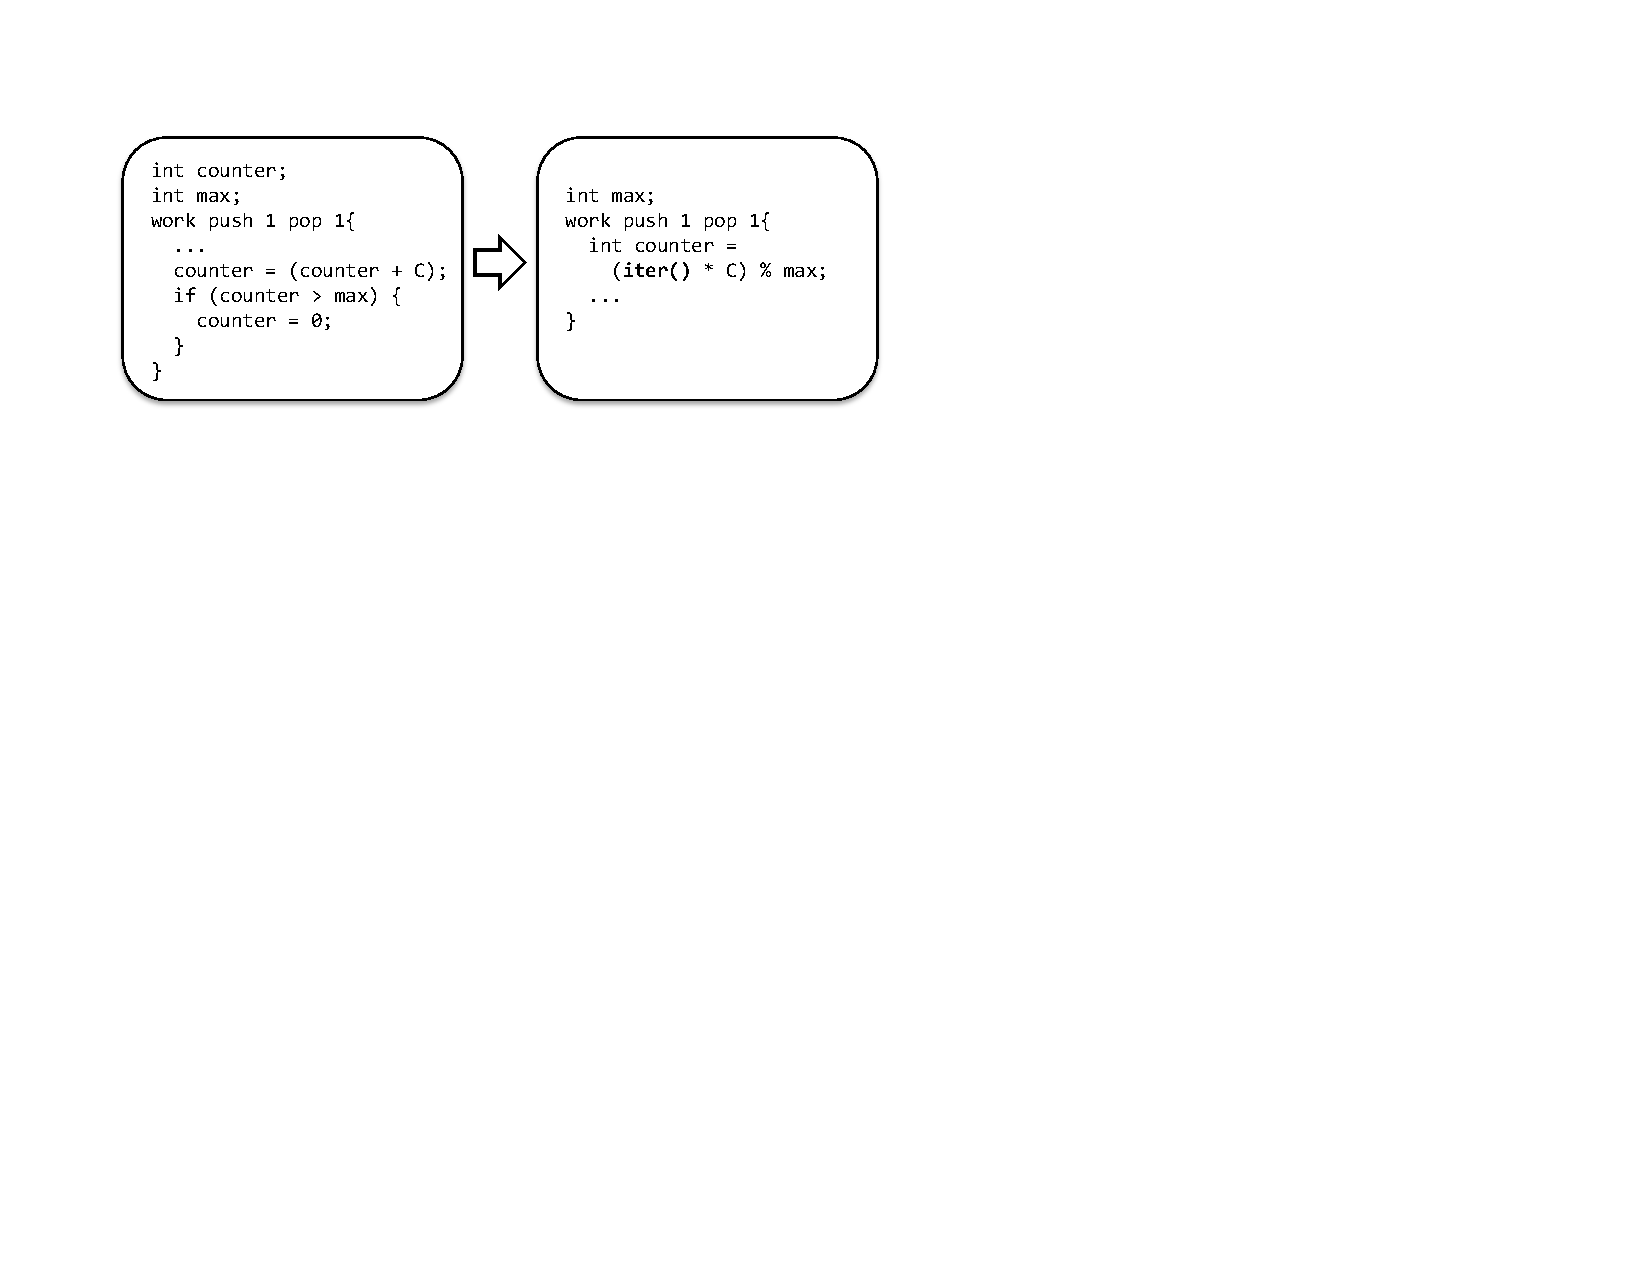
\includegraphics[width=3.5in]{figures/transformation1.pdf}
\caption{Translation of a simple filter with induction variable state that resets after a certain value. \protect\label{fig:transform-after-simple}}
\end{figure}

\begin{figure}[t]
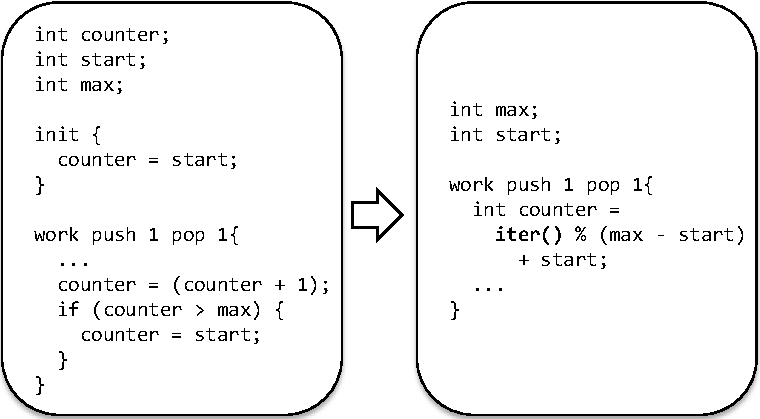
\includegraphics[width=3.5in]{figures/transformation2.pdf}
\caption{Translation of a simple filter with induction variable state that resets to a special value. \protect\label{fig:transform-after-start}}
\end{figure}

\begin{figure}[t]
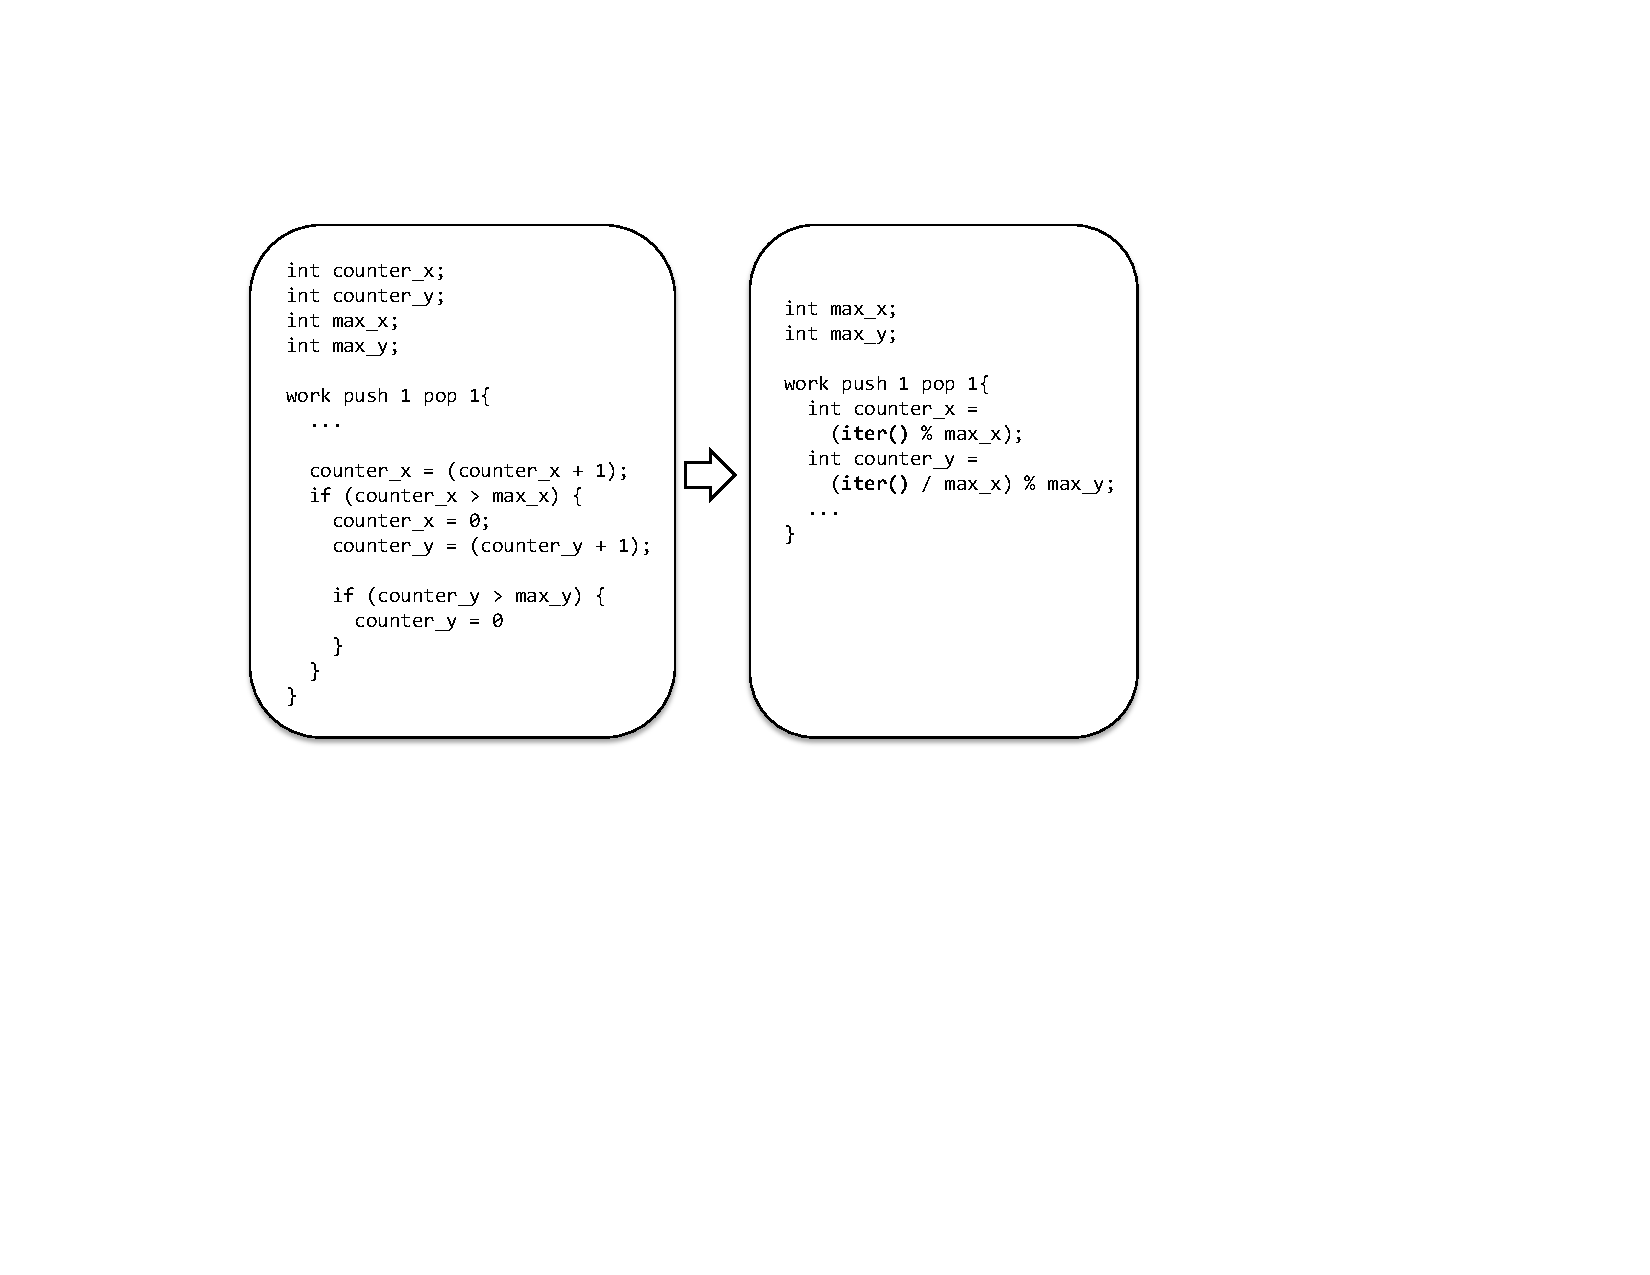
\includegraphics[width=3.5in]{figures/transformation3.pdf}
\caption{Translation of a filter with nested induction variables. \protect\label{fig:transform-after-twonested}}
\end{figure}

Programmers should not have to worry about how to introduce data parallelism into their programs.  With the introduction of a new language construct, hereafter referred to as {\tt iter()}, the programmer can take measures to write their programs to expose data parallelism.  Use of {\tt iter()} potentially provides further benefits in programmability and code readability as well.

The transformation from filters using induction variable state to using {\tt iter()} is fairly simple for users to implement.  Many of these transformations follow the same approach as induction variable elimination.  User defined induction variables can all be derived from the number of times the filter has been invoked.  Accordingly, the induction variable can be expressed as an arithmetic manipulation of {\tt iter()}.  

As described before, induction variable state requires the user to maintain mutable state, updating such state within the filter invocation, and potentially resetting them when required. The programmer can eliminate much of this code simply by arithmetically manipulating {\tt iter()} usage.  As an example, consider the stateful filter with induction state as defined in ~\ref{fig:transform-after-simple}.  The code necessary for maintaining the {\tt counter} field can all be eliminated using general induction variable elimination techniques.  

For filters that define multiple induction variables, it is possible to redefine these values in terms of {\tt iter()} as well.  It is not necessary to maintain multiple separate values for state.  Independent and nested induction variable state alike can be defined with use of {\tt iter()}.

This approach of using {\tt iter} to define induction variable state helps users write filters in a stateless manner.  The user can think about programming their filters in a stateless manner, and thereby exposing data parallelism. 


